\documentclass{article}
%%%%%%%%%%%%%%%%%%%%%%%%%%%%%%%%%%%%%%%%%%%%%%%%%%%%%%%%%%%%%%%%%%%%%%%%%%%%%%%%%%%%%%%%%%%%%%%%%%%%%%%%%
\usepackage{csquotes,xpatch}% recommended
\usepackage[backend=bibtex,
style=authoryear-comp,
sortcites=false,
maxbibnames=5,maxcitenames=2,
firstinits=true,
natbib=true,
]{biblatex}

\addbibresource{refs.bib}

% natbib = true: add comma between author and year
% firstinits: for first name initials in bibliography
\renewcommand{\postnotedelim}{ } % remove comma in post citation in autocite
%\addbibresource{refs.bib}
%%%%%%%%%%%%%%%%%%%%%%%%%%%%%%%%%%%%%%%%%%%%%%%%%%%%%%%%%%%%%%%%%%%%%%%%%%%%%%%%%%%%%%%%%%%%%%%%%%%%%%%%%

% Combine label and labelyear links
\xpatchbibmacro{cite}
{\usebibmacro{cite:label}%
	\setunit{\addspace}%
	\usebibmacro{cite:labelyear+extrayear}}
{\printtext[bibhyperref]{%
		\DeclareFieldAlias{bibhyperref}{default}%
		\usebibmacro{cite:label}%
		\setunit{\addspace}%
		\usebibmacro{cite:labelyear+extrayear}}}{}{}

% Include labelname in labelyear link
\xpatchbibmacro{cite}
{\printnames{labelname}%
	\setunit{\nameyeardelim}%
	\usebibmacro{cite:labelyear+extrayear}}
{\printtext[bibhyperref]{%
		\DeclareFieldAlias{bibhyperref}{default}%
		\printnames{labelname}%
		\setunit{\nameyeardelim}%
		\usebibmacro{cite:labelyear+extrayear}}}{}{}

% Access hyperref's citation link start/end commands
\makeatletter
\protected\def\blx@imc@biblinkstart{%
	\@ifnextchar[%]
	{\blx@biblinkstart}
	{\blx@biblinkstart[\abx@field@entrykey]}}
\def\blx@biblinkstart[#1]{%
	\blx@sfsave\hyper@natlinkstart{\the\c@refsection @#1}\blx@sfrest}
\protected\def\blx@imc@biblinkend{%
	\blx@sfsave\hyper@natlinkend\blx@sfrest}
\blx@regimcs{\biblinkstart \biblinkend}
\makeatother

\newbool{cbx:link}

% Include parentheses around labelyear in \textcite only in
% single citations without pre- and postnotes
\def\iflinkparens{%
	\ifboolexpr{ test {\ifnumequal{\value{multicitetotal}}{0}} and
		test {\ifnumequal{\value{citetotal}}{1}} and
		test {\iffieldundef{prenote}} and
		test {\iffieldundef{postnote}} }}

\xpatchbibmacro{textcite}
{\printnames{labelname}}
{\iflinkparens
	{\DeclareFieldAlias{bibhyperref}{default}%
		\global\booltrue{cbx:link}\biblinkstart%
		\printnames{labelname}}
	{\printtext[bibhyperref]{\printnames{labelname}}}}{}{}

\xpatchbibmacro{textcite}
{\usebibmacro{cite:label}}
{\iflinkparens
	{\DeclareFieldAlias{bibhyperref}{default}%
		\global\booltrue{cbx:link}\biblinkstart%
		\usebibmacro{cite:label}}
	{\usebibmacro{cite:label}}}{}{}

\xpretobibmacro{textcite:postnote}
{\ifbool{cbx:link}% patch 2.7+
	{\ifbool{cbx:parens}
		{\bibcloseparen\global\boolfalse{cbx:parens}}
		{}%
		\biblinkend\global\boolfalse{cbx:link}}
	{}}
{}
{\xpatchbibmacro{textcite}% patch earlier releases
	{\setunit{%
			\ifbool{cbx:parens}
			{\bibcloseparen\global\boolfalse{cbx:parens}}
			{}%
			\multicitedelim}}
	{\ifbool{cbx:link}
		{\ifbool{cbx:parens}
			{\bibcloseparen\global\boolfalse{cbx:parens}}
			{}%
			\biblinkend\global\boolfalse{cbx:link}}
		{}%
		\setunit{%
			\ifbool{cbx:parens}
			{\bibcloseparen\global\boolfalse{cbx:parens}}
			{}%
			\multicitedelim}}
	{}{}}
%%%%%%%%%%%%%%%%%%%%%%%%%%%%%%%%%%%%%%%%%%%%%%%%%%%%%%%%%%%%%%%%%%%%%%%%%%%%%%%%%%%%%%%%%%%%%%%%%%%%%%%%%
\DeclareNameAlias{sortname}{last-first} % last name first
\renewbibmacro{in:}{} % remove in: before journal

%%%%%%%%%%%%%%%%%%%%%%%%%%%%%%%%%%%%%%%%%%%%%%%%%%%%%%%%%%%%%%%%%%%%%%%%%%%%%%%%%%%%%%%%%%%%%%%%%%%%%%%%%
\usepackage{graphicx}
\usepackage{epstopdf} 
%%%%%%%%%%%%%%%%%%%%%%%%%%%%%%%%%%%%%%%%%%%%%%%%%%%%%%%%%%%%%%%%%%%%%%%%%%%%%%%%%%%%%%%%%%%%%%%%%%%%%%%%%
\usepackage{calrsfs}
\usepackage{physics}
\usepackage{mathtools}  
\usepackage{amsmath}
\usepackage{amssymb}
\usepackage{tabulary}
\usepackage{booktabs}
\usepackage{hyperref}
%%%%%%%%%%%%%%%%%%%%%%%%%%%%%%%%%%%%%%%%%%%%%%%%%%%%%%%%%%%%%%%%%%%%%%%%%%%%%%%%%%%%%%%%%%%%%%%%%%%%%%%%%
%\usepackage{chngcntr}
%\numberwithin{equation}{chapter}
%\counterwithin{figure}{chapter}
%%%%%%%%%%%%%%%%%%%%%%%%%%%%%%%%%%%%%%%%%%%%%%%%%%%%%%%%%%%%%%%%%%%%%%%%%%%%%%%%%%%%%%%%%%%%%%%%%%%%%%%%%
\setlength{\parindent}{2em}
\setlength{\parskip}{1em}

\linespread{1.6}
\usepackage{geometry}
\geometry{
	a4paper,
	total={134mm,225mm},
	left=38mm,
	top=35mm,
	headsep=.5in
}
\raggedbottom
%%%%%%%%%%%%%%%%%%%%%%%%%%%%%%%%%%%%%%%%%%%%%%%%%%%%%%%%%%%%%%%%%%%%%%%%%%%%%%%%%%%%%%%%%%%%%%%%%%%%%%%%%
\usepackage{blindtext}
\usepackage{ragged2e}
\usepackage{float}

\usepackage{epstopdf}
\usepackage{empheq} 

\usepackage{array}
\hypersetup{
	colorlinks
}
%%%%%%%%%%%%%%%%%%%%%%%%%%%%%%%%%%%%%%%%%%%%%%%%%%%%%%%%%%%%%%%%%%%%%%%%%%%%%%%%%%%%%%%%%%%%%%%%%%%%%%%%%
\usepackage{graphics}
\graphicspath{ {figures/} }
\renewcommand{\listfigurename}{List of figures}

\usepackage[labelfont=bf,justification=justified,singlelinecheck=false]{caption}
\captionsetup[figure]{name=Fig. ,labelsep=period}
\captionsetup[table]{labelsep=period}
\captionsetup[figure]{labelfont={bf},labelformat={default},labelsep=period,name={Fig.}}
%%%%%%%%%%%%%%%%%%%%%%%%%%%%%%%%%%%%%%%%%%%%%%%%%%%%%%%%%%%%%%%%%%%%%%%%%%%%%%%%%%%%%%%%%%%%%%%%%%%%%%%%%
\usepackage{array}
\usepackage{longtable}
\usepackage{xcolor}

\usepackage{comment}

\usepackage{enumitem}

\usepackage{wrapfig}
%%%%%%%%%%%%%%%%%%%%%%%%%%%%%%%%%%%%%%%%%%%%%%%%%%%%%%%%%%%%%%%%%%%%%%%%%%%%%%%%%%%%%%%%%%%%%%%%%%%%%%%%%
\usepackage{titlesec}

\titlespacing*{\section}
{0pt}{1ex plus .5ex minus .2ex}{.5ex plus .2ex}
\titlespacing*{\subsection}
{0pt}{0.5ex plus .5ex minus .2ex}{.5ex plus .2ex}
%\titlespacing*{\subparagraph}
%{0pt}{2.5ex plus 1ex minus .2ex}{1.3ex plus .2ex}

\setcounter{secnumdepth}{4}
\setcounter{tocdepth}{4}

\newcommand{\hsp}{\hspace{5pt}}

\titleformat{\section}[block]{\bfseries\large}{\thesection}{1em}{}
\titleformat{\subsection}[block]{\bfseries\itshape}{\thesubsection}{1em}{}


%\titleformat{\subsubsection}
%{\normalfont\normalsize\itshape}{\thesubsubsection}{1em}{}
%\titleformat{\subparagraph}[runin]
%{\itshape\normalsize}{\thesubparagraph}{1em}{}

%%%%%%%%%%%%%%%%%%%%%%%%%%%%%%%%%%%%%%%%%%%%%%%%%%%%%%%%%%%%%%%%%%%%%%%%%%%%%%%%%%%%%%%%%%%%%%%%%%%%%%%%%
\usepackage{subcaption}
\usepackage{bbm}
\usepackage{tabularx}
%%%%%%%%%%%%%%%%%%%%%%%%%%%%%%%%%%%%%%%%%%%%%%%%%%%%%%%%%%%%%%%%%%%%%%%%%%%%%%%%%%%%%%%%%%%%%%%%%%%%%%%%%
\definecolor{mycolor}{RGB}{207,42,40}
\AtBeginDocument{\hypersetup{citecolor=violet, linkcolor = mycolor}}

\usepackage{indentfirst}


%%%%%%%%%%%%%%%%%%%%%%%%%%%%%%%%%%%%%%%%%%%%%%%%%%%%%%%%%%%%%%%%%%%%%%%%%%%%%%%%%%%%%%%%%%%%%%%%%%%%%%%%
\setlength{\belowcaptionskip}{-20pt}


\usepackage{enumitem}
\usepackage{amsmath,bm}
\usepackage{graphicx}

\DeclareMathAlphabet{\pazocal}{OMS}{zplm}{m}{n}

\usepackage[ruled,vlined]{algorithm2e}
\SetKwComment{Comment}{$\triangleright$\ }{}
\newenvironment{problem_algorithm}[1][htb]
{\renewcommand{\algorithmcfname}{Algorithm for Problem}% Update algorithm name
	\begin{algorithm}[#1]%
	}{\end{algorithm}}

\usepackage{hyperref}

\begin{document}
	
	\sloppy
	
%%%%%%%%%%%%%%%%%%%%%%%%%%%%%%%%%%%%%%%%%%%%%%%%%%%%%%%%%%%%%%%%%%%%%%%%%%%%%%%%%%%%%%%%%%%%%%%%%%%%%%%%%
	\begin{center}	
		\Large
		\textbf{Evidential classification/regression}\\
		\large
%		\today
	\end{center}
	\vskip 0.5in
	
%%%%%%%%%%%%%%%%%%%%%%%%%%%%%%%%%%%%%%%%%%%%%%%%%%%%%%%%%%%%%%%%%%%%%%%%%%%%%%%%%%%%%%%%%%%%%%%%%%%%%%%%%
{\footnotesize
	\setlength{\parskip}{0.1em}
	\linespread{0.1}
	\tableofcontents}

\newpage
\section{Parameter estimation}\label{sec:estimation}
\subsection{Bernoulli/Categorical distribution}
Consider an i.i.d dataset $\pazocal{D} = \{y_i\}_{i=1}^{N}$, where each $y_i$ can take values from $\{1, 0\}$ and is sampled from a Bernoulli distribution with unknown probability $\mu$. 
This can describe a series of coin tosses and the objective is to estimate the underlying probability of ``Heads'' occurrence.
Let's denote Heads with the outcome $1$.  
The data likelihood for this binary variable experiment is given as
\begin{equation}
	p(\pazocal{D}|\mu) = \prod_{i=1}^{N}\mu^{y_i}(1-\mu)^{1-y_i}\
\end{equation}
and the maximum likelihood estimate (MLE) is given as 
\begin{equation}
	\mu_{MLE} = \frac{N_H}{N}
\end{equation}
where $N_H$ is the number of Heads in the $N$ samples. 
The MLE is thus the sample mean and we can use it for making future predictions.
However, if for example after 3 tosses we observe 3 Heads, then $\mu_{MLE} = 1$, i.e., it predicts that the next sample will be Heads with probability 1. 
This is an extreme case of overfitting. 

More generally, for describing quantities that can take $K$ possible values we can use a categorical distribution (also referred to as Multinoulli) with an unknown vector of discrete class probabilities $\mu = [\mu_1,\dots, \mu_K]^T$ which sums to 1; i.e., it belongs to the $K-1$-simplex.
The MLE for this set of parameters is given as $\mu_{MLE} = [N_1/N,\dots, N_K/N]^T$. 

In binary classification problems, for each $x$ the class $y(x)$ is typically modeled with a Bernoulli distribution and in multi-class classification problems for each $x$ the class $y(x)$ is typically modeled with a categorical distribution.

\subsection{Gaussian distribution}
Consider a i.i.d. dataset $\pazocal{D} = \{y_i\}_{i=1}^{N}$, where each $y_i$ can take values in $\mathbb{R}$ and is sampled from a Gaussian distribution with unknown mean $\mu$ and variance $\sigma^2$. 
The data likelihood for this experiment is proportional to
\begin{equation}
	p(\pazocal{D}|\mu, \sigma^2) \propto \prod_{i=1}^{N} exp\left(-\frac{(y_i-\mu)^2}{2\sigma^2}\right)
\end{equation}
and the MLE as 
\begin{equation}
	\mu_{MLE} = \bar{y} = \frac{1}{N}\sum{y_i} \text{, } \ 
	\sigma^2_{MLE} = \frac{1}{N}\sum{(y_i - \bar{y})^2}
\end{equation}
The MLE for $\sigma^2$ is biased and is typically corrected by multiplying by $\frac{N}{N-1}$. 
This is because both $\mu$ and $\sigma^2$ are estimated from the data.

In regression problems, for each $x$ the variable $y(x)$ is typically modeled with a Gaussian distribution.

\subsection{Bayesian inference}
MLE gives only point estimates of the parameters of interest and can lead to overfitted results for small datasets. 
In this regard, the Bayesian framework treats the unknown parameters as random variables with associated probabilities corresponding to degrees of belief. 
Thus, for a parameter set $w$ (this may refer to the $\mu$ vector in categorical or $\{\mu, \sigma^2\}$ in Gaussian distribution), instead of maximizing the likelihood $p(\pazocal{D}|w)$ and obtaining a point estimate $w_{MLE}$, we introduce a posterior probability distribution $p(w|\pazocal{D})$ which specifies the plausibility of each value for $w$ based on the data. 
The posterior is given as
\begin{equation}\label{eq:posterior}
	p(w|\pazocal{D}, \eta) = \frac{p(\pazocal{D}|w)p(w, \eta)}{p(\pazocal{D, \eta})}
\end{equation}
where $p(w, \eta)$ is a prior distribution for the parameters and $\eta$ represents a set of hyperparameters (e.g., the prior variance).
Note that the likelihood may have its own hyperparameters as well.

If we obtain the posterior $p(w|\pazocal{D}, \eta)$ we can use it to make future predictions. 
But how do we obtain the posterior?
We observe that the posterior is proportional to the product of the likelihood and the prior, i.e., 
\begin{equation}
	p(w|\pazocal{D}, \eta) \propto p(\pazocal{D}|w)p(w, \eta)
\end{equation}
Therefore, if we can introduce a prior that interacts in an analytically convenient manner with the likelihood then we can obtain the posterior analytically. 
This is the case for conjugate priors. 
Such priors interact with the likelihood in such a way so that the posterior and the prior belong to the same probability distribution family. 

Interestingly, for any likelihood function belonging to the exponential family (such as the Bernoulli, categorical and Gaussian distributions), there exists a conjugate prior and we also have its functional form.
For example, the conjugate prior for the Bernoulli likelihood is the Beta distribution, for the categorical the Dirichlet distribution and for the Gaussian with unknown mean and variance the normal-inverse-Gamma (NIG) distribution.

As a result, we can obtain analytically the posterior for such cases. 
For a Bernoulli likelihood the prior is Beta$(\mu|\alpha, \beta)$ and the posterior is Beta$(\mu|\alpha+N_H, \beta+N_T)$. 
Next, for a categorical likelihood the prior is Dirichlet$(\mu|\alpha)$, where $\alpha = [\alpha_1,\dots, \alpha_K]^T$, and the posterior is Dirichlet$(\mu|\alpha + [N_1,\dots, N_K]^T)$. 
Finally, for a Gaussian likelihood the prior is NIG$(\mu, \sigma^2|\gamma, v, \alpha, \beta)$ and the posterior is NIG$(\mu, \sigma^2|g(\gamma, v, \alpha, \beta, \bar{y}, \sum(y_i-\bar{y})^2))$ where $g$ is a known function (see \textcite{bishop2006pattern}).
Overall, the posterior is fully specified by the prior and the sufficient statistics of the data. 

\subsection{Prior/Posterior predictive}
After obtaining the posterior we would like to make predictions. 
Before any data had arrived the predictions could be based only on the prior; this is the prior predictive distribution given as
\begin{equation}\label{eq:prior:predictive}
	p(y|\eta) = \int p(y|w)p(w|\eta) dw
\end{equation}
or, equivalently, 
\begin{equation}\label{eq:prior:predictive:2}
	prior \ predictive (y|\eta) = \int likelihood(y|w) \times prior(w|\eta) dw
\end{equation}
For example, for the categorical/Dirichlet pair the prior predictive is 
\begin{equation}\label{eq:prior:predictive:dirichlet}
	p(y|\eta) = \int \prod_{j=1}^{K}\mu_j^{y_j} \times Dirichlet(\mu|\eta)d\mu
\end{equation}
which degenerates to $p(y = \lambda|\eta) = \eta_{\lambda} / \sum_k\eta_j$.
For the Gaussian/NIG pair the prior predictive is
\begin{equation}\label{eq:prior:predictive:nig}
	p(y|\eta) = \int Gaussian(y|\mu, \sigma^2)\times NIG(\mu, \sigma^2|\eta)d\mu d\sigma^2
\end{equation}
which is expressed as a Student-t distribution that depends on $\eta$.

After the data has arrived we can incorporate it for making predictions; this is the posterior predictive given as
\begin{equation}\label{eq:posterior:predictive}
	p(y|\eta, \pazocal{D}) = \int p(y|w)p(w|\eta, \pazocal{D}) dw
\end{equation}
or, equivalently, 
\begin{equation}\label{eq:posterior:predictive:2}
	posterior \ predictive (y|\eta, \pazocal{D}) = \int likelihood(y|w) \times posterior(w|\eta, \pazocal{D}) dw
\end{equation}
Recall that the prior $p(w|\eta)$ and the posterior $p(w|\eta, \pazocal{D})$ have the same functional form due to conjugacy. 
Therefore, the analytical closed-form expressions we have for Eq.~\eqref{eq:prior:predictive} (Eqs.~\eqref{eq:prior:predictive:dirichlet}-\eqref{eq:prior:predictive:nig}) apply to Eq.~\eqref{eq:posterior:predictive} as well with minimal changes. 

Finally, note that the hyperparameters $\eta$ can be estimated from type-II MLE (also known as empirical Bayes), i.e., by maximizing the marginal likelihood $p(\pazocal{D}|\eta)$. 
The marginal likelihood is given as
\begin{equation}\label{eq:marginal:likelihood}
	p(\pazocal{D}|\eta) = \int p(\pazocal{D}|w)p(w|\eta) dw
\end{equation}

\subsection{Prior hyperparameters as fictitious evidence}\label{sec:fictitious:evidence}
Conjugacy has two more implications. 
First, the posterior predictive can be construed as a prior predictive with better-informed prior hyperparameters and can be used as the prior when subsequent data arrives.
In this regard, the posterior hyperparameters are a function of the prior ones and the sufficient statistics of the data; say $\tilde{\eta} = g(\eta, s(\pazocal{D}))$.
They incorporate the ``evidence'' provided by the data $\pazocal{D}$.
Second, following the same rationale, the prior hyperparameters $\eta$ can be construed as ``pseudo-evidence'', i.e., corresponding to some fictitious observations.

For example, $\alpha$, $\beta$ of the Beta prior can be interpreted as fictitious observations of $\alpha$ Heads and $\beta$ Tails in a coin tossing experiment.
Similarly for the Dirichlet prior. 
For the NIG prior the hyperparameters $\gamma$, $v$ can be interpreted as $v$ fictitious observations with sample mean $\gamma$ and the hyperparameters $\alpha$, $\beta$ as $2\alpha$ observations with sample mean $\gamma$ and sum of square residuals $2\beta$.

This is a general result for exponential distributions: hyperparameters can be interpreted as corresponding to fictitious observations.

\subsection{Why the introduction}
The term ``evidential'' in evidential classification/regression refers to this fictitious evidence corresponding to the prior hyperparameters. 
To elaborate further, consider the following extreme scenario: suppose we have no data (i.e., no access to a posterior predictive), but somehow have very good prior hyperparameters $\eta$. 
Then we can use the prior predictive for making predictions with accuracy depending on the number of fictitious observations the hyperparameters $\eta$ correspond. 

In evidential classification/regression the parameters $\eta$ for each $x$ are produced by a neural network (NN). 
It is, thus, \textit{as if the NN produced the corresponding fictitious evidence}. 
Finally, for predicting $y(x)$ the prior predictive is used with hyperparameters given by the NN output $\eta(x)$. 

\section{Classification/Regression}
\subsection{Problem description}

In the standard binary classification setting the likelihood for the value $y(x)$ for every $x$ can be modeled as a Bernoulli distribution, i.e., 
\begin{equation}\label{eq:class:likelihood}
	p(y|x, w) = Bernoulli(y|\mu_w(x))
\end{equation}
where the vector of probabilities $\mu_w(x)$ (e.g., $[0.8, 0.2]$) can be the output of a NN.
The prediction $y^*(x)$ is typically taken as the class corresponding to the maximum probability in $\mu_w(x)$.
Similarly for multi-class classification with a categorical instead of a Bernoulli distribution.

In the regression setting the likelihood for $y(x)$ for every $x$ can be modeled as a Gaussian distribution, i.e., 
\begin{equation}\label{eq:regression:likelihood}
	p(y|x, w) = Gaussian(y|\mu_w(x), \sigma^2_w(x) \text{ or }  \sigma^2)
\end{equation}
where the aleatoric uncertainty variance is either considered as a hyperparameter $\sigma^2$ or is also part of the NN output.
Typically, if a single prediction value is required it can be given as $y^*(x) = \mu_w(x)$.

For fitting the aforementioned NNs and estimating the model parameters $w$, the MLE can be used. 
For classification, MLE corresponds to minimizing the cross-entropy loss, whereas for regression, MLE corresponds to minimizing the sum of squared errors loss.
However, MLE leads to overfitting and thus, regularized MLE is used instead (which can be seen as a MAP estimate). 

Nevertheless, these approaches provide only point estimates. 
Even if we estimate aleatoric uncertainty through $\sigma^2$ or $\sigma_w^2(x)$ we still have no estimate for epistemic uncertainty, i.e., uncertainty related to estimating the model parameters $w$.
For example, we would like to have an estimate for the variance of $\mu_w(x)$.

\subsection{Bayesian treatment}

The Bayesian treatment of classification/regression is briefly discussed here in order to draw a distinction between the Bayesian and the evidential frameworks.

In this regard, predictions are made using the posterior predictive of Eqs.~\eqref{eq:posterior:predictive}-\eqref{eq:posterior:predictive:2}. 
The likelihood $p(y|w)$ used in these equations is given by Eq.~\eqref{eq:class:likelihood} for classification and by Eq.~\eqref{eq:regression:likelihood} for regression, and the posterior $p(w|\eta, \pazocal{D})$ is given by Eq.~\eqref{eq:posterior}.


In realistic settings the posterior predictive is approximated with a Monte Carlo (MC) estimate as
\begin{equation}\label{eq:posterior:predictive:mc}
	p(y|x, \eta, \pazocal{D}) = \int p(y|x, w)p(w|\eta, \pazocal{D}) dw \approx 
	\frac{1}{M}\sum_{j = 1}^{M}p(y|x, \hat{w}_j)
\end{equation}
with $\{\hat{w}_j\}_{j=1}^{M}$ sampled from the posterior $p(w|\eta, \pazocal{D})$.
The prior hyperparameters $\eta$ correspond to the prior of the $w$ parameters which are the NN parameters. 
They do not correspond to the prior of the likelihood parameters as in Section 1. 
The likelihood parameters are given as the output of the NN (e.g., $\mu_w(x)$ for the Gaussian).

As an example, for regression we can obtain the following estimates:
\begin{table}[H]
	\centering
	\begin{tabular}{ | c | c | c  |} 
		\hline
		Mean function & $\mathbb{E}[\mu(x)]$ & $\frac{1}{M}\sum_{j=1}^{M}\mu_{\hat{w}_j}(x)$ \\
		\hline
		Epistemic uncertainty & $Var[\mu(x)]$ & $Var\left[\{\mu_{\hat{w}_j}(x)\}_{j=1}^{M}\right]$\\
		\hline
		Aleatoric uncertainty & $\mathbb{E}[\sigma^2]$ & $\frac{1}{M}\sum_{j=1}^{M}\sigma^2_{\hat{w}_j}(x)$ or $\sigma^2$ \\
			\hline
	\end{tabular}
	\caption{Interpretation of Bayesian regression estimates.}
	\label{tab:bayes:regression}
\end{table}

The main limitation of the Bayesian framework is that it is not straightforward to produce samples $\{\hat{w}_j\}_{j=1}^{M}$ from the posterior.
Posterior approximation techniques, depending on their accuracy, are computationally costly.

Finally, note that that the hyperparameters $\eta$ can be estimated by type-II MLE, i.e., by maximizing the marginal likelihood of Eq.~\eqref{eq:marginal:likelihood}.

\subsection{Evidential treatment}
\subsubsection{Introduction}\label{sec:evidential:intro}
In the deterministic framework we consider a likelihood function for each $x$ with parameters given by a NN which is itself parametrized. 
For example, our prediction for $y(x)$ in the regression setting is a Gaussian likelihood with mean given by a NN.
And by optimizing the NN parameters we obtain the likelihood parameters.

In the Bayesian framework the same is considered except for the fact that many different values for the NN parameters are averaged in an MC fashion.
The hyperparameters $\eta$ in the Bayesian framework correspond to the prior of the NN parameters and do not depend on the location $x$. 

The evidential treatment is completely orthogonal to the above.
Instead of making predictions using the likelihood we make predictions using the prior predictive of Eqs.~\eqref{eq:posterior:predictive}-\eqref{eq:posterior:predictive:2}. 
The hyperparameters $\eta$ of the prior predictive are given by the output of the NN and depend on the location $x$. 
Overall, there are three main differences with the Bayesian framework:
\begin{enumerate}
	\item For each $x$ instead of using the likelihood with parameters given by a NN, we use the prior predictive with hyperparameters $\eta$ given by a NN
	\item In the Bayesian framework $\eta$ corresponds to the prior of the NN parameters and is shared among all $x$ locations, whereas in the evidential framework it corresponds to the prior of the likelihood parameters and varies depending on $x$
	\item We deterministically optimize the evidential NN (with regularized MLE).
	However, epistemic uncertainty is already embedded in the prior predictive distribution so we do have an estimate for it.
\end{enumerate}

\subsubsection{Making predictions}
As explained in Section~\ref{sec:evidential:intro}, for each $x$ the prior predictive is used for predicting $y(x)$.
The required hyperparameters $\eta(x)$ are given as the output of a NN. 

Specifically, for the classification setting, the prior predictive is given by Eq.~\eqref{eq:prior:predictive:dirichlet} and the required hyperparameters $\eta = [\alpha_1, \dots, \alpha_K]$ are given by the sum of $[1, \dots, 1]$ and the output of a NN; i.e., $[1, \dots, 1]$ represents the totally uncertain state, whereas the NN represents the additional (fictitious) evidence.
This sum is also the vector of probabilities for $x$ belonging in each class.

For the regression setting, the prior predictive is a Student-t distribution (derived from Eq.~\eqref{eq:prior:predictive:nig}) and the required hyperparameters $\eta = [\gamma, v, \alpha, \beta]$ are given by a NN; i.e., the NN outputs 
\begin{equation}
	\eta_w(x) = \begin{bmatrix}
		\gamma_w(x) \\ v_w(x) \\ \alpha_w(x) \\ \beta_w(x)
	\end{bmatrix}
	= \begin{bmatrix}
		\gamma \\ v \\ \alpha \\ \beta
	\end{bmatrix}
\end{equation}
These hyperparameters have the following interpretations:
\begin{table}[H]
	\centering
	\begin{tabular}{ | c | c | c  |} 
		\hline
		Mean function & $\mathbb{E}[\mu(x)]$ & $\gamma$ \\
		\hline
		Epistemic uncertainty & $Var[\mu(x)]$ & $\frac{\beta}{v(\alpha - 1)}$\\
		\hline
		Aleatoric uncertainty & $\mathbb{E}[\sigma^2]$ & $\frac{\beta}{\alpha - 1}$\\
		\hline
	\end{tabular}
	\caption{Interpretation of evidential regression output.}
	\label{tab:evidential:regression}
	\end{table}
As also mentioned earlier, epistemic uncertainty is already embedded in the output of the prior predictive; thus it is not affected by the fact that we deterministically optimize our NN).
See Fig.~\ref{fig:standard:vs:evidential} for a sketch of the evidential regression NN outputs as compared to the one of standard regression NN.
\begin{figure}[H]
	\centering
	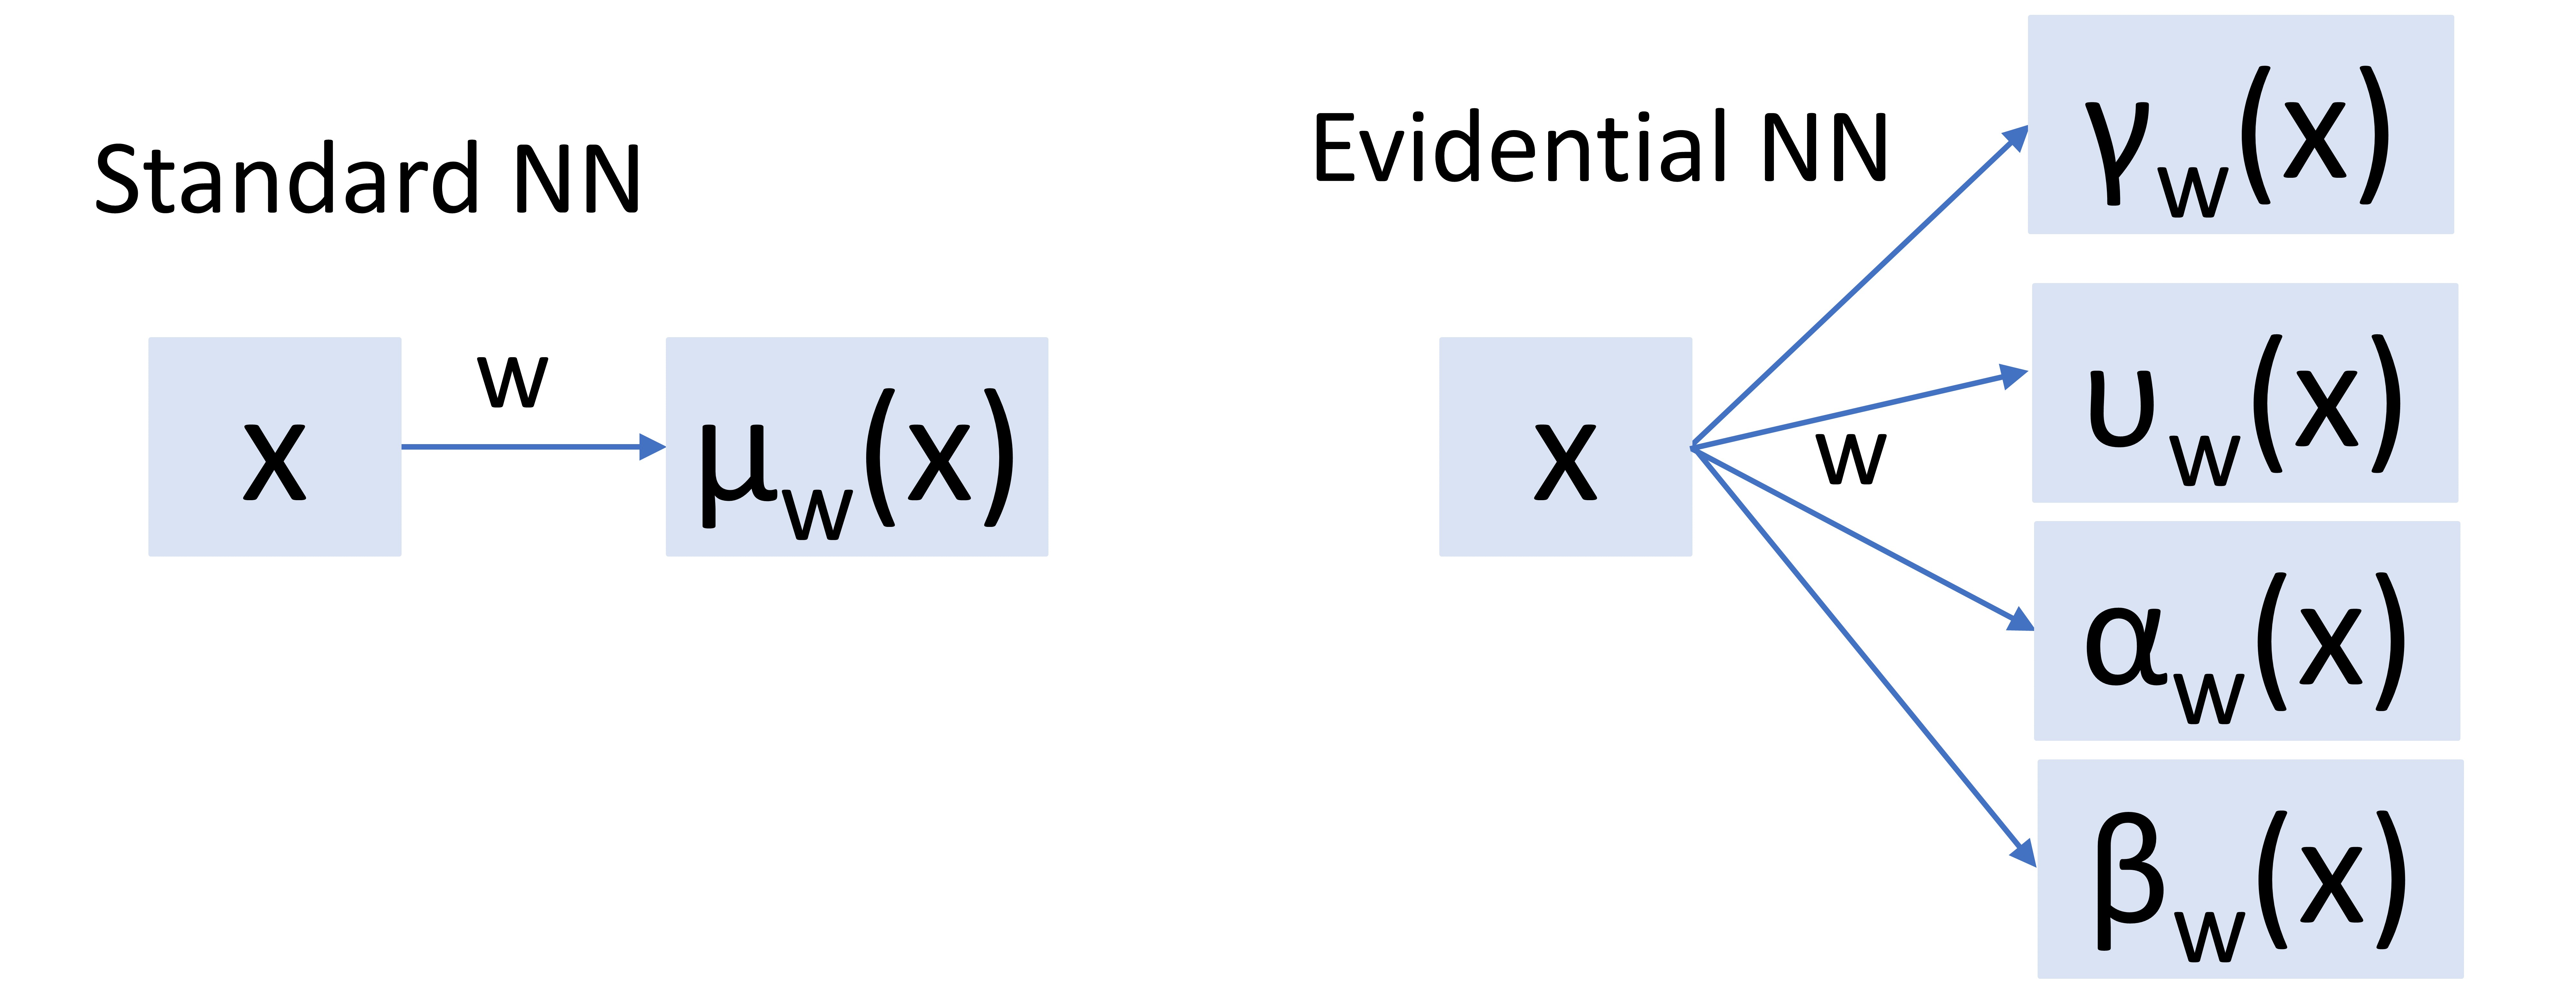
\includegraphics[width=.85\linewidth]{./figs/standard_vs_evidential.jpg}
	\caption{Standard vs evidential NN outputs.}
	\label{fig:standard:vs:evidential}
\end{figure}

According to the original paper \textcite{amini2020deep}, the evidential distribution (the prior predictive) can be construed as a higher-order distribution on top of the unknown lower-order likelihood distribution from which observations are drawn. 
As depicted in Fig.~\ref{fig:evidential:distribution}-A, different values of fictitious evidence output by the NN correspond to different higher-order distributions. 
And based on NN-predicted higher-order distribution (Fig.~\ref{fig:evidential:distribution}-B), different likelihood functions can be drawn as shown in Fig.~\ref{fig:evidential:distribution}-C.
\begin{figure}[H]
	\centering
	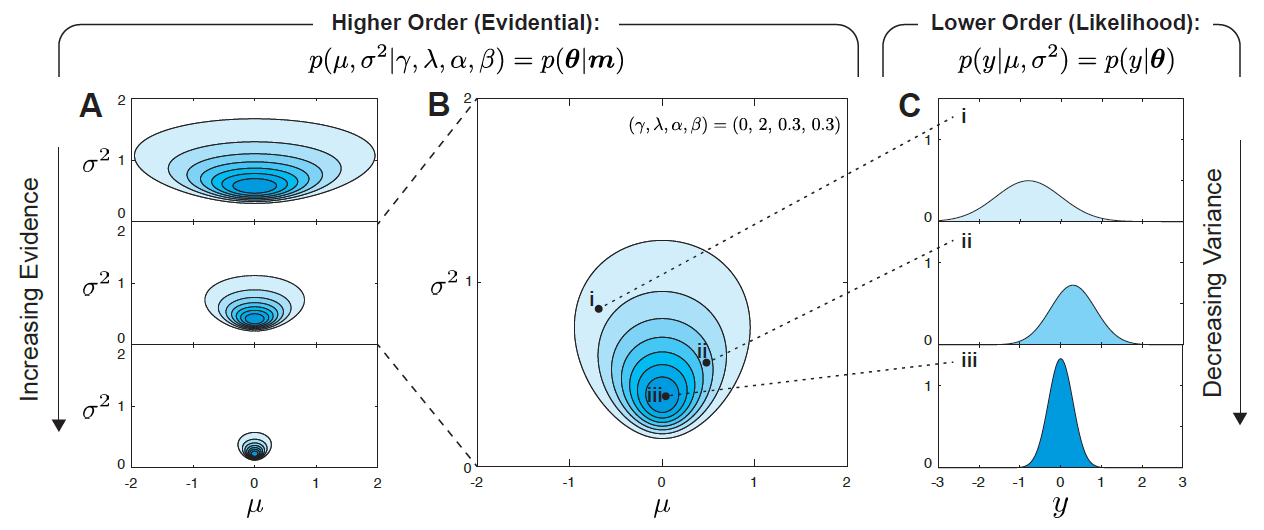
\includegraphics[width=.85\linewidth]{./figs/evidential_distributions.png}
	\caption{According to the original paper \textcite{amini2020deep}, the evidential distribution (the prior predictive) can be construed as a higher-order distribution on top of the unknown lower-order likelihood distribution from which observations are drawn. 
		As depicted in part A of the figure, different values of fictitious evidence output by the NN correspond to different higher-order distributions. 
		And based on NN-predicted higher-order distribution (part B), different likelihood functions can be drawn as shown in part C.}
	\label{fig:evidential:distribution}
\end{figure}

\subsubsection{Loss function for evidential learning}
As explained in previous sections, in the Bayesian framework the hyperparameters $\eta$, which parametrize the prior of the NN parameters and are shared among $x$ locations, are tuned with type-II MLE (marginal likelihood maximization). 
In this regard, recall the typical interpretation of marginal likelihood: it is the probability for the dataset to occur under the prior predictive. 
For this reason, the marginal likelihood can also be used for defining a loss function for evidential training, in which predictions are based on the prior predictive.
As a result, the loss function can be expressed as
\begin{equation}\label{eq:evidential:loss}
	Loss(w) = \sum_{i=1}^{N} -log [p(y_i|\eta_w(x_i))]
\end{equation}
Because we have an analytical expression for $p(y_i|\eta_w(x_i))$ (Student-t for regression), it is straightforward to compute the loss corresponding to $w$.
Training with the loss function of Eq.~\eqref{eq:evidential:loss} can also be interpreted as standard MLE training with a Student-t likelihood instead of a Gaussian likelihood. 

For regularization, the approach proposed by \textcite{sensoy2018evidential} is to penalize the network for leaving the ``I do not know'' state; i.e., a change in $w$ should make a significant data misfit reduction, otherwise the NN output should correspond to large uncertainty. 
In evidential terms, large uncertainty corresponds to small fictitious evidence (see Section~\ref{sec:fictitious:evidence}). 

Specifically, for the Dirichlet prior the ``I do not know'' state corresponds to $\eta = [1, \dots, 1]$ which is a uniform prior that does not favor any one direction.
The penalty term for this case can be given as the KL divergence of the proposed prior Dirichlet$(\eta_w(x))$ from the totally uncertain prior Dirichlet$([1, \dots, 1])$. 
See \textcite{sensoy2018evidential} for more information regarding the classification case.

For the regression case, the KL divergence between the NN-produced NIG prior and the zero-evidence NIG prior is undefined (see \cite{amini2020deep}).
For proposing an alternative approach the following properties are desirable:
\begin{itemize}
	\item A larger penalty value should be applied for larger data misfit
	\item A larger penalty value should be applied for larger fictitious evidence. Recall that prior hyperparameters can be interpreted as fictitious evidence/observations (see Section~\ref{sec:fictitious:evidence}). 
	More evidence produced by the NN corresponds to less uncertainty and it is desirable this less uncertainty to be backed by significant reduction in data misfit.
\end{itemize} 
Based on the above properties, \textcite{amini2020deep} proposes the loss function to be regularized by 
\begin{equation}\label{eq:evidential:regularizer}
	R(w) = \sum_{i=1}^{N}|y_i-\gamma_w(x_i)|(2\alpha_w(x_i) + v_w(x_i))
\end{equation}
where $2\alpha_w(x_i) + v_w(x_i)$ is the total number of fictitius observations that are produced by the NN (see Section~\ref{sec:fictitious:evidence} for more information).
Note that in the first version of \textcite{amini2020deep} the total evidence is given as in Eq.~\eqref{eq:evidential:regularizer}, whereas in the second version it is given as $\alpha_w(x_i) + 2v_w(x_i)$, which should be a typo.

\subsection{Summary}

In Table~\ref{table:summary} the evidential regression framework is compared with standard regression. 
\begin{table}[H]
	\centering
	\begin{tabular}{ | c | c | c |}
		\hline
		\textbf{Regression / Training} & \textbf{Predictive function} & \textbf{Optimization} \\
		\hline
		Standard / MLE & $\pazocal{N}(y|\mu_{\hat{w}}(x), \sigma^2)$ & $\min_w \ \sum_{i=1}^{N}||y_i-\mu_w(x_i)||_2^2$ \\
		\hline
		 Standard / Reg. MLE & $\pazocal{N}(y|\mu_{\hat{w}}(x), \sigma^2)$ & 
		 \vtop{\hbox{\strut $\min_w \ \sum_{i=1}^{N}||y_i-\mu_w(x_i)||_2^2$}\hbox{\strut $+ \lambda||w||_2^2$}} \\
		\hline
		 Standard / Bayesian& $\frac{1}{M}\sum_{j=1}^{M} \pazocal{N}(y|\mu_{\hat{w}_j}(x), \sigma^2)$ & Posterior sampling \\
		 \hline
		 Evidential / Reg. MLE & $\textit{Student-t}(y|\eta_{\hat{w}}(x))$ & Eq.~\eqref{eq:evidential:loss} + Eq.~\eqref{eq:evidential:regularizer} \\
		\hline
	\end{tabular}
\caption{Evidential vs standard regression.}
\label{table:summary}
\end{table}

\section{Key points through examples}

A few key points based on the numerical examples of \textcite{amini2020deep} are summarized below: 
\begin{itemize}
	\item Evidential regression does not rely on sampling during prediction (also seen as ``inference'') and thus is faster than sampling-based alternatives (e.g., dropout, Bayes by backprop, HMC). 
	However, this cost may not be very significant in general. 
	\begin{figure}[H]
		\centering
		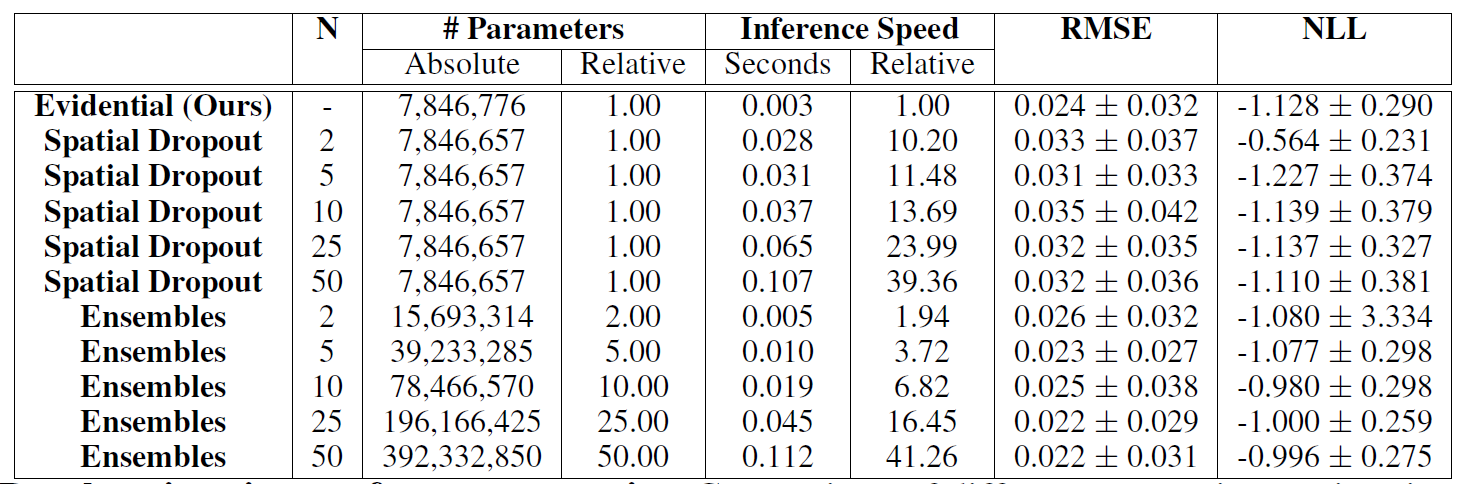
\includegraphics[width=1\linewidth]{./figs/inference_speed.png}
		\caption{Inference speed comparison for the depth estimation regression problem. See more info in \textcite{amini2020deep}.}
		\label{fig:inference:speed}
	\end{figure}

	\item Predicted epistemic uncertainty depends highly on the regularization parameter $\lambda$ of Eq.\eqref{eq:evidential:regularizer}, as opposed to aleatoric uncertainty
	\begin{figure}[H]
		\centering
		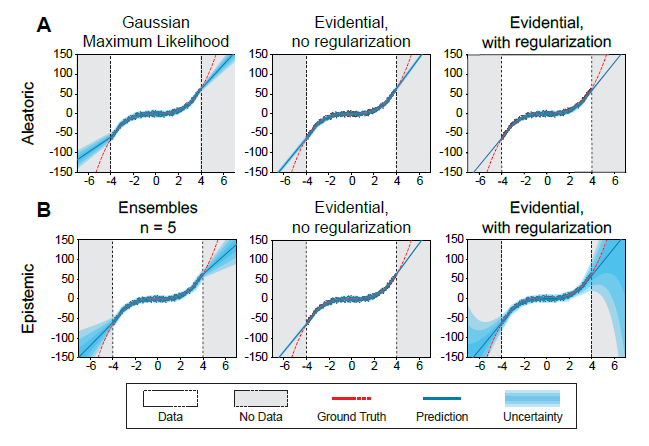
\includegraphics[width=.85\linewidth]{./figs/regularization.png}
		\caption{Effect of regularization for the cubic function regression problem.}
		\label{fig:regularization}
	\end{figure}	
	\item With the right $\lambda$ value evidential regression can give better predictions for out-of-distribution epistemic uncertainty as compared to Dropout and Deep Ensembles
	\begin{figure}[H]
		\centering
		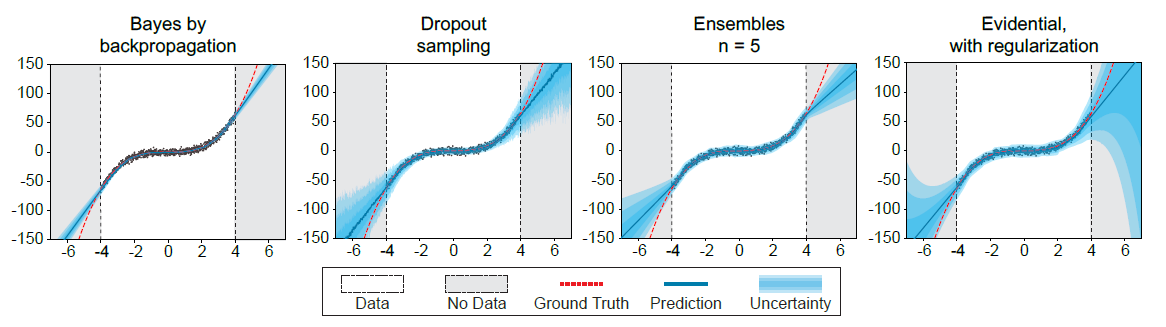
\includegraphics[width=1\linewidth]{./figs/uncertainty.png}
		\caption{Total uncertainty comparison for the cubic function regression problem.}
		\label{fig:uncertainty}
	\end{figure}
	\item Evidential regression is competitive both in terms of accuracy (RMSE) and uncertainty estimation (negative log-likelihood; NLL).
	Note that NLL although has a term that corresponds to sum of squared errors, it also has a term that relates to the predicted uncertainty and how the data agrees with this uncertainty
	\begin{figure}[H]
		\centering
		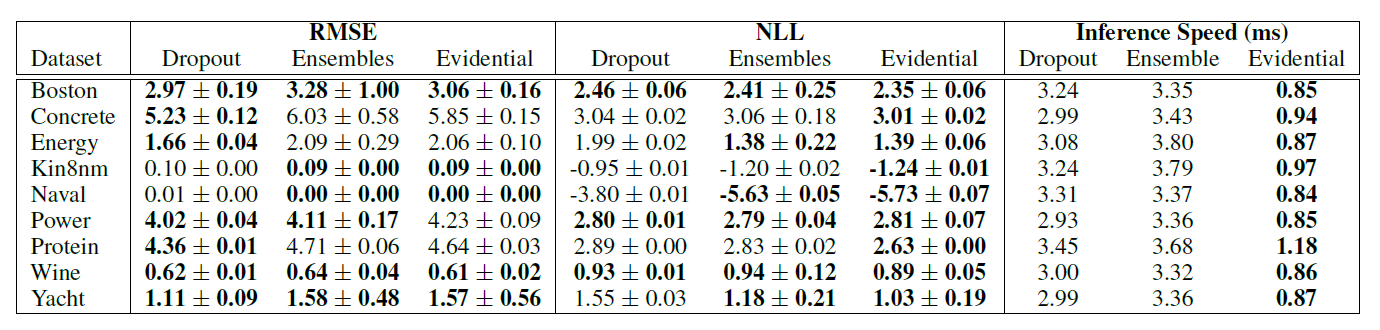
\includegraphics[width=1\linewidth]{./figs/accuracy.png}
		\caption{Accuracy and uncertainty comparison for benchmark regression problems.}
		\label{fig:accuracy}
	\end{figure}
	\item Evidential regression effectively disentangles epistemic and aleatoric uncertainties. 
	\begin{figure}[H]
		\centering
		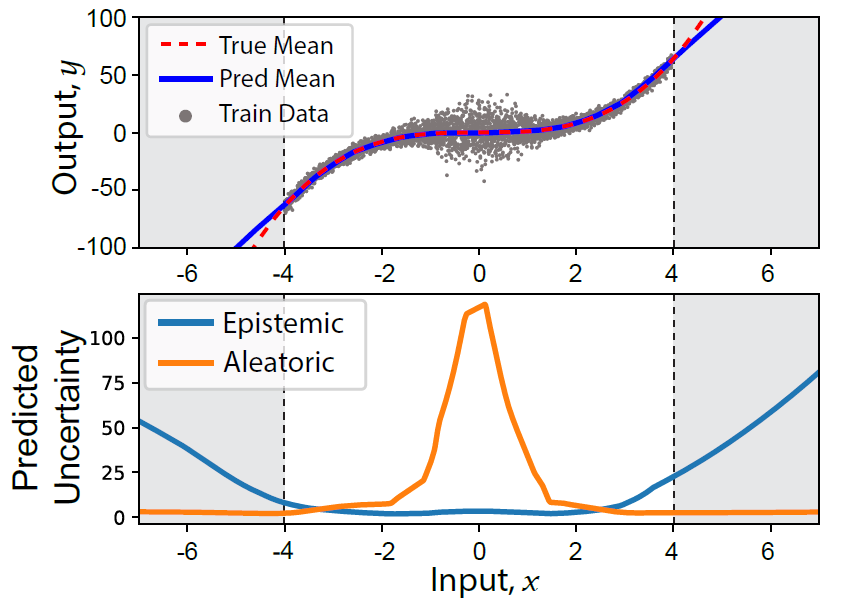
\includegraphics[width=.85\linewidth]{./figs/disentangled.png}
		\caption{Disentangled uncertainty for the cubic function regression problem with more added noise towards the center of the in-distribution region. 
		Predicted aleatoric uncertainty increases in the middle (as it should) and predicted epistemic uncertainty increases where there is no data (as it should).}
		\label{fig:disentangled}
	\end{figure}	
	
	
\end{itemize}









	


%%%%%%%%%%%%%%%%%%%%%%%%%%%%%%%%%%%%%%%%%%%%%%%%%%%%%%%%%%%%%%%%%%%%%%%%%%%%%%%%%%%%%%%%%%%%%%%%%%%%%%%%%	

%\section*{Appendix}
\newpage	
\printbibliography[heading=bibintoc,title={References}]
	
\end{document}